\section{Vorarbeiten}\label{kap:vorarbeiten}
Zu dieser Bachelor-Thesis gab es bereits eine Vorarbeit im letzten Semester. Diese hatte zum Ziel, einige
grundlegende Funktionalitäten bereitzustellen. In Abbildung \ref{fig:billiard_ai_cycle} ist der Zyklus angegeben,
welcher alle Aufgaben zusammenfasst. In einem ersten Schritt wird der aktuelle Spielstand über eine Kamera detektiert.
Daraus kann eine textuelle Beschreibung abgeleitet werden. Diese dient wiederum als Input für das Kernstück, die Suche
nach einem optimalen Stoss. Als Ausgabe dieses Schrittes erfolgt eine detaillierte Animation des auszuführenden Stosses.
Die Animation wird über einen Projektor auf dem Billardtisch dem Spieler zugänglich gemacht. Dieser kann den Stoss ausführen,
was zu einer neuen Situation führt und der Zyklus beginnt von vorne.

\begin{figure}[h!]
    \begin{center}
        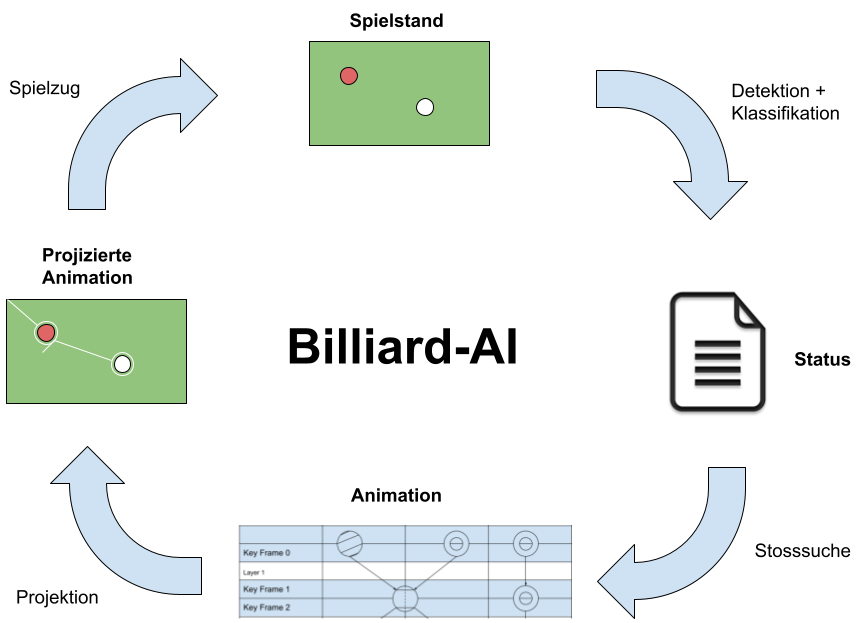
\includegraphics[width=0.8\linewidth]{../common/03_billiard_ai/resources/19_billiard_ai_cycle.png}
    \end{center}
    \caption{Billard-AI-Cycle}
    \label{fig:billiard_ai_cycle}
\end{figure}

Es sind nun die Schritte der Detektion des Spielstands wie auch die Projektion und Darstellung der Animation auf dem
Spieltisch bereits umgesetzt. Dabei ging es in erster Linie um die Frage der Repräsentation in geeignetem Koordiantensystem
sowie die Messung der Genauigkeit dieser Übersetzung und der darauf basierenden Anzeige über den Projektor.

Die Bachelor-Thesis widmet sich zuerst der Frage nach der Klassifikation in Schritt eins, wie auch der Suche
nach dem optimalen Stoss in Schritt zwei.